\documentclass[a4paper]{book}

%% Language and font encodings
\usepackage[T1,T8K,T8M]{fontenc}
\usepackage[utf8]{inputenc}
\usepackage[english,georgian]{babel}

%% Sets page size and margins
\usepackage[a4paper,top=3cm,bottom=2cm,left=3cm,right=3cm,marginparwidth=1.75cm]{geometry}

\usepackage[plainpages=false,bookmarksopen,pdfpagelabels, %
pdftex,
pdfproducer={Latex with hyperref},
pdfcreator={pdflatex},
bookmarksnumbered,unicode]{hyperref} 



%% Useful packages
\usepackage{amsmath}
\usepackage{graphicx}
\usepackage[colorinlistoftodos]{todonotes}
%\usepackage[colorlinks = true, allcolors = blue]{hyperref}
\usepackage{float}
\usepackage{enumerate}
\usepackage{subfig}
\usepackage{gensymb}
\usepackage{rotating}
\usepackage[version=4]{mhchem}


\title{ფიზიკა}
\author{ლევან კანკაძე}

\begin{document}
\maketitle

\tableofcontents

\chapter{წინასიტყვაობა.}
აქ არის მოგროვებული სხვადასხვა მასალები ფიზიკაში.


\chapter{მექანიკა}

\section{ამოცანები}
ნივთიერი წერტილი იწყებს მოძრაობას წრფეზე $a$ მუდმივი აჩქარებით. $t_1$ დროის შემდეგ აჩქარება იცვლის ნიშანს, და მოდულით იგივე რჩება.
განსაზღვრეთ რა $t$ დროის შემდეგ დაუბრუნდება იგი საწყისს წერტილს.

%\begin{turn}{180}
პასუხი: $t = t_1(2 + \sqrt{2})$
%\end{FlushLeft}

მატარებელი იმყოფებოდა $L = 400$ მ შუქნიშიდან და ქონდა სიჩქარე $v = 45$ კმ/სთ, როცა დაიწყო დამუხრუჭება. 
განსაზღვრე ლოკომოტივის მდებარეობა შუქნიშნის მიმართ 1 წუთის შემდეგ, მოძრაობდა $a = 3$

პასუხი: 25 მ

\section{4 ვექტორი}
%Griffiths, David J. - Introduction to Elementary Particles [2nd Edition]

\section{რეაქტიული მოძრაობა}

\section{სტატიკა} სტატიკაში შეისწავლება მყარი სხეულების წონასწორობა, რომელზეც მოქმედებს ძალები. წონასწორობაში იგულისხმება მდგომარეობა, რომლისთვისაც, სხეულს არ გააჩნია აჩქარება, ანუ მოძრაობს თანაბრად და წრფივად, ან ნაწილობრივ, იმყოფება უძრავად ათვლის ინერციულ სისტემაში. (პრაქტიკულად ამოცანებში, დედამიწასთან დაკავშირებული ათვლის სისტემა ითვლება ინერციულად).

განვიხილოთ თუ რა ძალები მოქმედებს წონასწორობაში მყოფ სხეულზე. პირველ რიგში უნდა გავიხსენოთ სიმძიმის ძალა. ეს სიმძიმის ძალა არის ტოლქმედი სხეულის შემადგენელი ნაწილაკების სიმძიმის ძალისა. სიმძიმის ძალა გადის სხეულის მასათა ცენტრზე. 
	
შემდეგ მოქმედებს ბმის რეაქციის ძალები - ეს ძალები ეწინააღმდეგება სხეულის მოძრაობას რომელიმე მიმართულებით. ბმის რეაქციის ძალა მიმართულია იმ მიმართულების საწინააღმდეგოდ, რომელი მიმართულებითაც ბმა ეწინააღმდეგება სხეულის მოძრაობას. რეაქციის ძალებია - დრეკადობისა და ხახუნის ძალები. მათი მოდულები და ზოგჯერ მიმართულება წინასწარ არაა ცნობილი და დამოკიდებულია, სხეულის ფორმაზე, ზედაპირების მდგომარეობაზე, ასევე სხეულზე მოქმედ სხვა ძალებზე.
	
რეაქციის ძალის მიმართულების განსაზღვრა აუცილებელია სტატიკის ამოცანების სწორად ამოსახსნელად.	

ამიტომაც განვიხილოთ როგორაა მიმართული რამდენიმე სახის ბმის რეაქციის ძალები:
	
1. 
	
2. გადაბმა არის დრეკადი ძაფით ან უმასო ღეროთი, ძაფის შემთხვევაში დრეკადობის ძალა არის ყოველთვის მიმართული ძაფის გასწვრივ და "გამოდის" იმ წერტილიდან რომლითაც მიმაგრებულია სხეულზე ან ხდება გადაბმა. ღეროს დრეკადობის ძალის შემთხვევაში იგულისხმება იმ ძალის მნიშვნელობა რომლითაც ღერო იჭიმება ან იკუმშება, თუ ღერო უმასოა მაშინ აღძრული ძალა მიმართული იქნება ღეროს გასწვრივ, ხოლო მიმართულება (გამოდის თუ შედის ძალა გადაბმის წერტილში) უნდა დავადგინოთ ამოცანის პირობით.
%		\begin{figure}[H]
%	 	\centering
%           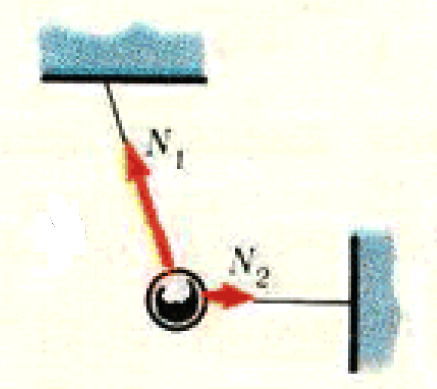
\includegraphics[width=0.2\columnwidth]{figures/static_c}
%           \caption{ძაფის შემთხვევა.}
%           \label{fig:static_c}
%        \end{figure}
		\begin{figure}[H]%
   			 \centering
   			 \subfloat[\centering ძაფის შემთხევა]{{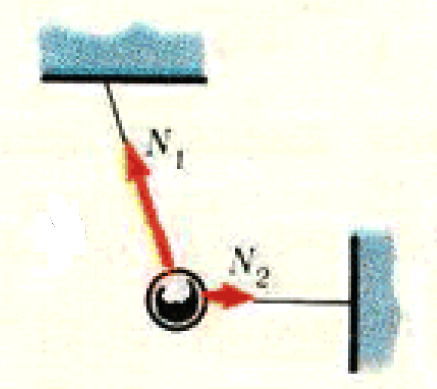
\includegraphics[width=5cm]{figures/static_c} }}%
    		\qquad
    		\subfloat[\centering ღეროს შემთხვევა]{{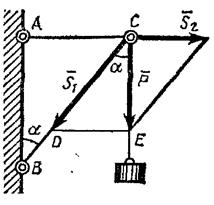
\includegraphics[width=5cm]{figures/static_b} }}%
   	 		\caption{ძალები}%
    	\label{fig:example}%
		\end{figure}	 
	 
3. სახსრული შეერთება - 


\textbf{ამოცანა} თხელი ერთგვაროვანი ღერო სახსრულადაა დამაგრებული წერტილ $A$-ში. ღეროს მეორე ბოლო კედელზე ძაფითაა დამაგრებული, ისე როგორც ნახაზზეა \ref{fig:statics_1}  ნაჩვენები. ღეროს მასაა $m = 1$ კგ, ღერო ჰორიზონტისადმი დახრილია $\alpha = 45 \degree$. იპოვეთ სახსარში აღძრული დრეკადობის ძალა. 
	 	\begin{figure}[H]
	 	   \centering
           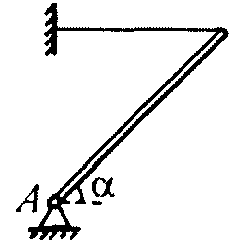
\includegraphics[width=0.2\columnwidth]{figures/statics_1}
           \caption{ამოცანა.}
           \label{fig:statics_1}
        \end{figure}

\section{შენახვის კანონები დაჯახებებში}

\section{მასათა ცენტრი}
მექანიკის ამოცანების ამოხსნისას, მატერიალურ წერტილთა სისტემის მასათა ცენტრის მცნების გამოყენებამ, შეიძლება ფასდაუდებელი დახმარება გაგვიწიოს. ზოგიერთი ამოცანის ამოხსნა საგრძნობლად მარტივდება და თვალსაჩინო ხდება, ხოლო ზოგიერთის ამოხსნა საერთოდ შეუძლებელია მისი გამოყენების გარეშე. სანამ შევუდგებით კონკრეტული ამოცანების ამოხსნას, დავიხსომოთ ძირითადი მასათა ცენტრის თვისებები, რომლების ილუსტრირებული იქნება კონკრეტული მაგალითებით.

მატერიალურ წერტილთა სისტემის მასათა ცენტრი (ინერციის ცენტრი) ვუწოდოთ წერტილს, რომელიც ახასიათებს სისტემაში მასის განაწილებას და რომლის კოორდინატებიც მოიცემა ფორმულებით
	\begin{equation}
		x_{\text{მც}} = \frac{m_1x_1 + \dotsb + m_Nx_N}{m_1 + \dotsb + m_N} \quad
		y_{\text{მც}} = \frac{m_1y_1 + \dotsb + m_Ny_N}{m_1 + \dotsb + m_N} \quad
		z_{\text{მც}} = \frac{m_1z_1 + \dotsb + m_Nz_N}{m_1 + \dotsb + m_N} \quad
	\end{equation}
$m_i$ - მატერიალური წერტილების მასებია, $x_1,y_i,z_i$ - ამ წერტილების კოორდინატებია. თუ მკითხველისათვის ცნობილია რადიუს ვექტორის მცნება, ზემოთ მოყვანილი სისტემა შეიძლება ჩაიწეროს, ერთ ვექტორულ ტოლობად:
	\begin{equation}
		r_{\vec{\text{მც}}} = \frac{m_1\vec{r_1} + \dotsb + m_N\vec{r_N}}{m_1 + \dotsb + m_N}
	\end{equation}
გავარჩიოთ რამდენიმე ამოცანა:\\
\textbf{ამოცანა 1} ვიპოვოთ მარტივი სისტემის მასათა, ცენტრი რომელიც შედგება ორი წერტილისაგან მასებით $m_1$ და $m_2$ და მათ შორის მანძილია $l$.


\subsection{ამოცანები.}
\textbf{ამოცანა} ცილინდრული ღეროს ერთი ნახევარი თუთიისა , მეორე ნახევარი - ალუმინის. განსაზღვრეთ სისტემის მასათა ცენტრის მდებარეობა, თუ ღეროს სიგრძე 40 სმ-ია.

\textbf{ამოცანა} თუთიისა და ალუმინის ერთნაირი მოცულობის ორი ბირთვი შეერთებულია შეხების წერტილით. განსაზღვრეთ სისტემის მასათა ცენტრი.

\textbf{ამოცანა} 3 და 5 მასის ორი სფერო მიმაგრებულია 2 კგ მასის და 30 სმ სიგრძის ღეროს ბოლოებზე. სფეროს რადიუსებია, შესაბამისად, 5 და 7 სმ. განსაზღვრეთ სისტემის მასათა ცენტრი.

\textbf{ამოცანა}  ხუთი სფერო, რომელთა მასა მიმდევრობით 1, 2, 3, 4, 5, კგ-ის ტოლია, დამაგრებულია ღეროზე ისე, რომ მათი ცენტრები ერთმანეთისაგან, თანაბარი მანძილებითაა დაშორებული. უგულებელყავით ღეროს მასა და გაიგეთ სისტემის მასათა ცენტრი.

\textbf{ამოცანა} ერთგვაროვანი $R$ რადიუსის წრიული ფორმის თხელი ფირფიტიდან ორჯერ ნაკლები რადიუსის წრე ისეა ამოჭრილი, რომ ფირფიტის კიდეს ეხება. განსაზღვრეთ დარჩენილი ფიგურის მასათა ცენტრი.

\textbf{ამოცანა} ერთგვაროვანი $R = 105.6$ სმ წრიული ფორმის თხელი წრიდან ამოჭრილია კვადრატი ისე, როგორც სურათზეა გამოსახული.
განსაზღვრეთ დარჩენილი ფიგურის მასათა ცენტრი.

\textbf{ამოცანა} იპოვეთ მდებარეობს ერთგვაროვანი, თხელი მავთულისგან შეკრული სამკუთხედის მასათა ცენტრი.

\textbf{ამოცანა} ათი ბურთულა, რომელთა მასებია 1,2,...,10
გ. დამაგრებულია უმასო 90 სმ სიგრძის ღე-
როზე, ისე რომ ყოველ ბურთულას შორის მან-
ძილია 10 L1, განსაზღვრეთ მასათა ცენტრის
მდებარეობა

\textbf{ამოცანა} ერთგვაროვანი თხელი $R$ რადიუსის დისკოდან ამოჭრეს ორჯერ პატარა რადიუსის წრე, რომელიც ეხება წრეწირის ნაპირს. განსაზღვრეთ მასათა ცენტრის მდებარეობა. (სურათი საჭიროა)

\textbf{ამოცანა} სად მდებარეობს ერთგვაროვანი კუბის მასათა ცენტრი, თუ მისგან ამოჭრილია $a/2$ გვერდის მქონე კუბი. (სურათი საჭიროა)

 

5 - ოთხი ერთგვაროვანი ბურთი მასებით 7»
1 კგ, »% = 92 კგ, იკ =7 კგ, 3 კგ დამაგრე-
ბულია უწონო ღეროზე ისე როზ მათი ცენტრები
ერთამენითისაგან დაშორებულები არიან თანა-
ბარი მანძილით ძ = 0.2 მ. რა > მანძილითაა.
დაშორებული სისტემის მასათა ცენტრი მესამე

ბურთულას ცენტრიდან.

 
    

 

        

 

%6 - ტოლგვერდა სამკუთხედის ფორმის მავთუ-
%ლის ბარჩოს ორი გვერდი დამზადებულია ალუ-
%მინის მავთულისაგან, ხოლო მესამე სპილენ-
%მავთულის ნაჭრებს აქვთ ერთნაირი
%განიკვეთის ფართობი. სამკუთხეღის გვერდია
%L = 1 მ. ალუმინის სიმკკრივეა ი) = 2700 კგ/მ",
%სპილენძის #2 = 8900 კგ/მ1. იპოვოთ 72: მაჩწძილი

%მასათა ცენტრიდან სპილენძის მავ-

 

%ძისაგან.

 

 

 

 

%სისტემის
%თულის შუა წერტილამოე
%7 - ერთგვაროვან თხელ 7? რადიუსის დისკო-
%ზე ამოჭრილია ნახვრეტი რადიუსით » 7
%რომლის ცენტრიც /ჯ/2 მანძილითაა დაშორებუ-
%ლი დისკის ცენტრის. რა > მანძილზე იმყოფება
%დისკის ცენტრის ამ სისტემის მასათა ცენტრი ?

%“რე.
%ყყის |
%|

%ჩ

 

 

 

 

%ლ”

%8 - » რადიუსის მქონე ნასევარწრის ფორმის ერ-
%თგვაროვანი ფირფიტა შეერთებულია მართკუ-
%თხედთან სიგრძით 2» და სიგანით #. იპოვეთ
%#/I ისეთი შეფარდება, რომლისთვისაც სისტე-
%მის მასათა ცენტრი დაემთხვევა ნახევარწრის
%გეომეტრიულ C” ცენტრს. მანძილი ნახევარწრის
%მასათა C, ცენტრს და გეომეტრიულ C ცენტრს
%შორის მანძილი ტოლია 4» /(3»).

 



	\section{შენახვის კანონები}
	\textbf{01.} $m$ მასის უძრავ ბირთვს $V$ სიჩქარით ეჯახება $M$ მასის მოძრავი ბირთვი. იპოვეთ ბირთვების სიჩქარეები დაჯახების შემდეგ, თუ დაჯახება დრეკადია და ცენტრული. ძალის მოქმედებს წრფე გადის სხეულის მასათა ცენტრზე - სიმძიმის ცენტრი.
		
	\section{ჭოჭონაქები}
	\textbf{01.} იპოვეთ რა ძალით მოქმედებს ჭერზე, ნახატზე გამოსახული უმასო ჭოჭონაქების სისტემა. თოკები უჭიმვადია და უმასო,  თითოეული სხეულის მასაა $m$.  ხახუნი უგულებელყავით.
	 			\begin{figure}[H]
	 			\centering
           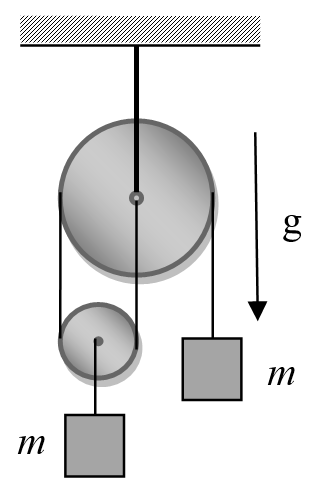
\includegraphics[width=0.2\columnwidth]{figures/03}
           \caption{A boat.}
           \label{fig:wowonaqi}
        \end{figure}

\section{კინემატიკური ბმები დინამიკის ამოცანებში}
%Черноуцан А., Кинематические связи в задачах динамики
მექანიკის ამოცანებში ხშირად გვხდება სიტუაცია, როდესაც სხეულის მოძრაობა არ არის თავისუფალი. ეს შეზღუდვა შეიძლება იყოს განპირობებული მყარი ზედაპირებით, უჭიმვადი ძაფებით, ხისტი ღეროებით და ასე შემდეგ. მარტივ შემთხვევებში ამ შეზღუდვებს ვითვალისწინებთ ავტომატურად და არც კი ვსაუბრობთ მასზე. მაგალითად სხეულის აჩქარებას პირდაპირ მივმართავთ სიბრტყის გასწვრივ (ცხადია მყარი ზედაპირის შემთხვევაში), ბუქსირზე ჩაბმული მანქანისა და მაბუქსირებელი მანქანის სიჩქარეს ვთვლით ტოლად (ვგულისხმობთ რომ მანქანები გადაბმულია უჭიმვადი ტროსით). ხანდახან კი აუცილებელია ეს შეზღუდვა აღვწეროთ სპეციალური განტოლებების საშუალებით, რომელთაც ჩვენ ვუწოდებთ \textbf{კინემატიკურ ბმას}. განვიხილოთ რამდენიმე ამოცანა.
%\begin{figure}
%\centering
%\begin{minipage}{.5\textwidth}
%  \centering
%  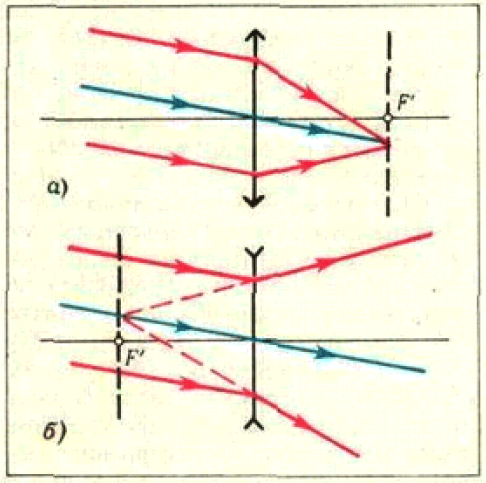
\includegraphics[width=.9\linewidth]{figures/optics_2}
%  \captionof{figure}{სხივთა სვლა თხელ ა) შემკრებ, ბ) გამბნევ ლინზაში.}
%  \label{fig:optics_1}
%\end{minipage}%
%\begin{minipage}{.5\textwidth}
%  \centering
%  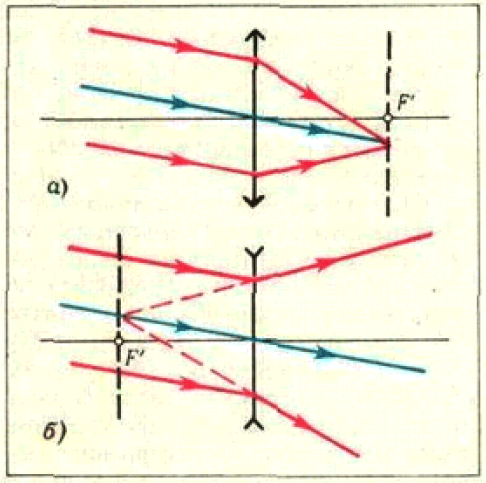
\includegraphics[width=.9\linewidth]{figures/optics_2}
%  \captionof{figure}{ლინზაზე დაცემულ პარალელურ სხივთა სვლა თხელ ა) შემკრებ, ბ) გამბნევ ლინზაში.}
%  \label{fig:optics_2}
%\end{minipage}
%\end{figure}
 
 
\section{მოძრაობა მოსახვევში}
\subsection{ამოცანები}
%გედენიძე 1010
\textbf{ამოცანა.} როგორი უნდა იყოს გზის პროფილი, რომ ავტომობილმა, მოსახვევში სიჩქარის შეუმცირებლად და უსაფრთხოდ მოუხვიოს?

%გედენიძე 1011
\textbf{ამოცანა.} გზის ჰორიზონტალურ უბანზე 140 მ რადიუსის წრეწირის 309-იანი რკალის დასაწყისში ავტომობილი ყველა წამყვანი 1.“
ალით იწყებს მოძრაობას და ზრდის სიჩქარის მოდულს. როგორ,
ჩაქსიმალური სიჩქარით შეუძლია გავიდეს ავტომობილი გზის წრ,
უბანზე? გზის ვაკისთან ბორბლების ხახუნის კოეფიციენტი 0,3.

%გედენიძე 1012
\textbf{ამოცანა.} გზის ჰორიზონტალურ უბანზე 140 მ რადიუსის მოსახვევში 14 ტ. მატარებლის ვაგონის სიჩქარე 18 კმ/სთ-ია. განსაზღვრეთ, რა ძალით მოქმედებს რელსი ვაგონის რებორდზე? გარე თუ შიდა რელსი მოქმედებს ბორბალზე? 3

+ 1013. ჯერ შეაფასეთ, შემდეგ განსაზღვრეთ, რამდენჯერ შეიცვ.
ღება რებორდზე მოქმედი ძალის მოდული მატარებლის ვაგონის
სიჩქარის ორჯერ გაზრდისას? შეადარეთ ერთმანეთს რელსის რე-
ორდზე და რებორდის რელსზე მოქმედი ძალები.

1014. 800მ რადიუსის სიმრუდის მოსახვევში მატარებელი მოძრაობს.
'0მ/წმ სიჩქარით. რამდენით მაღლა უნდა იყოს გარე რელსი შიდაზე,
ჩომ თვლების რებორდები არ ახღენღენ გვერდით დაწოლას რელსე-
ზე? ლიანდაგის სიგანეა 1534მმ.

1015. თქვენი ვარაუდით, რატომ ამცირებს მემანქანე მატარებლის
იჩქარის მოდულს მოსახვევში?

1016. მოციგურავე მოძრაობს 42მ რადიუსის წრეწირზე მოდუ-
ლით 12მ/წმ სიჩქარით. ჰორიზონტისადმი რა კუთხით უნდა გადაიხ-
როს იგი წონასწორობის შესანარჩუნებლად?

1017. რა მაქსიმალური სიჩქარით შეუძლია იმოძრაოს მოტო-
იკლმა გზის ჰორიზონტალურ უბანზე 90მ რადიუსის სიმრუდის
ოსახვევში, თუ სრიალის ხახუნის კოეფიციენტია 0,4? რას უნდა
ედრიდეს ამ დროს შვეულიდან გადახრა?

1018. რა მაქსიმალური სიჩქარით შეუძლია იმოძრაოს მოტო”
აიკლმა 309 -იანი კუთხით დახრილ ტრეკზ; ი შემოწერს 909
ჩადიუსის წრეწირს? ხახუნის კოეფიციენტი  0:4-ია.  · ,

% 1019. სეფი ა“ია.. ჯრ
არაერთი იმობილის. მგზავრი მოსახვევში მოხვევის. საბი“

. თ; „თქმის
ეუმჩნეველია. რვვეი“ 8 ავის მოხვევა კი მგზავრისათვის თითქ”

1020. თვითმფრინავი. ი.

უხვევს 6კმ რადიუსის წრეწირის რკალზე ?''

114


	 \textbf{01.} მოტოციკლეტისტი მოძრაობს ჰორიზონტალურ ზედაპირზე $v = 70$ კმ/სთ სიჩქარით, ბრუნდება $R = 100$ მ რადიუსის მოსახვევში, რა კუთხით უნდა გადაიხაროს რომ არ დაეცეს? \\
	 ამოხსნა\\
	 აქაც ხახუნის ძალაა, ძალა რომელიც აჩერებს მოტოციკლისტს, $F_{fr} = \frac{m v^2}{R}$, საყრდენის რეაქციის ძალა $N = mg$. მომენტების წესი სიმძიმის ცენტრის მიმართ მომცემს განტოლებას $F_{fr}\cdot l \sin \alpha = N l \cos \alpha$. აქ მოცემული არაა $\mu$ და მაგიტომ გვჭირდება. ეს მომენტები.
	 
	\textbf{02.} რა მაქსიმალური $v$ სიჩქარით შეიძლება იმოძრაოს მანქანამ $\alpha$ კუთხით დახრილ სიბრტყეზე თუ სიმრუდის რადიუსია $R$ და ხახუნის კოეფიციენტი ბორბლებსა და გზას შორის არის $k$.
			\begin{figure}[H]
           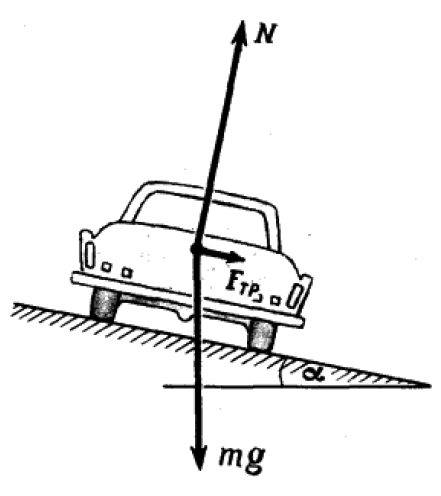
\includegraphics[width=0.2\columnwidth]{figures/02}
           \caption{A boat.}
           \label{fig:02}
        \end{figure}

%ბენდრიკოვი 301
განსაზღვრე პლანეტის $\rho$ საშუალო სიმკვრივე, თუ ეკვატორზე დინამომეტრზე ჩამოკიდებული ტვირთი $10~\%$-ით მსუბუქია ვიდრე პოლუსზე. დღეღამის ხანგრძლივობა პლანეტაზე $t = 6$ სთ-ია.

\section{მეშვიდე კლასი.}
ამოცანა ნომერი 4. ერთ ქვეყანაში გეოლოგმა იპოვა შავი მეტეორიტი
	 
\section{წრეწირზე მოძრაობა}
%Асламазов Л., Движение по окружности
წრეწირზე მოძრაობისას აღწერისას წრფივი სიჩქარის მცნებასთან ერთად შემოაქვთ კუთხური სიჩქარის განმარტებაც. თუკი ნივთიერი წერტილი წრეწირზე მოძრაობისას $\Delta t$ დროში შემოწერს რკალს, რომლის კუთხური ზომაა $\Delta \phi$, მაშინ კუთხური სიჩქარეა $\omega = \frac{\Delta \phi}{\Delta t}$.

\section{კოსმოსი}
\subsection{ნიუტონის გრავიტაციული ფორმულა}
ორი ნივთიერი წერტილი ერთმანეთს მიიზიდავს ძალით, რომელიც პირდაპირპროპორციულია მათი მასების ნამრავლისა და უკუპროპორციულია მათ შორის მანძილის კვადრატის.
	\begin{equation}
		F = G\frac{m_1 m_2}{r^2}
	\end{equation}
ანდა ჩაწერილი ვექტორული ფორმით.
	\begin{equation}
		\vec{F} = G\frac{m_1 m_2}{r^3}\vec{r}
	\end{equation}
$G = 6.67 \times 10^{-11} \dfrac{\text{ნ}\cdot\text{მ}^2}{\text{კგ}^2}$ კოეფიციენტს მსოფლიო მიზიდულობის ანუ გრავიტაციული მუდმივი ეწოდება.
ის პირველად ინგლისელმა ფიზიკოსმა ჰენრი კავენდიშმა განსაზღვრა ცდით.

\subsection{ელიფსი}%ნიკოს ნოუთები
ელიფსის ზოგიერთი თვისების შესწავლა დაგვეხმარება, ამოცანების ამოხსნაში, ამიტომაცაა აუცილებელი მისი ცოდნა.
	\begin{figure}[H]
	\centering
    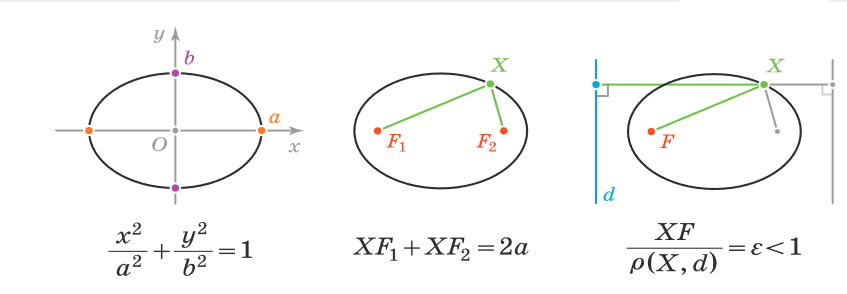
\includegraphics[width=0.9\columnwidth]{figures/ellipse}
    \caption{ამოცანა.}
    \label{fig:statics_1}
    %კვანტი 2021 12
    \end{figure}


\subsection{კეპლერის კანონები}%ნიკოს ნოუთები
\subsubsection{კეპლერის პირველი კანონი}
	პლანეტები მოძრაობს ელიფსებზე, რომელთა ერთ-ერთ ფოკუსში იმყოფება მზე.
\subsubsection{კეპლერის მეორე კანონი}
პლანეტის რადიუს-ვექტორი დროის ტოლ შუალედებში ტოლ ფართობებს მოხვეტს.
		\begin{figure}[H]
		   \centering
           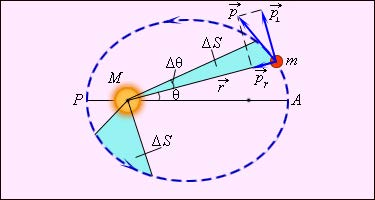
\includegraphics[width=0.5\columnwidth]{figures/kepler_2_law}
           \caption{კეპლერის მეორე კანონი - მოხვეტილი ფართობების ტოლობის კანონი.}
           \label{fig:kepler_2_law}
        \end{figure}
	
\subsubsection{კეპლერის მესამე კანონი}
	პლანეტების გარშემოვლის პერიოდების კვადრატები ისე შეეფარდება ერთმანეთს, როგორც მათი ორბიტების დიდი ნახევარღერძების კუბები.
	\begin{equation}
		\frac{T_1^2}{T_2^2} = \frac{a_1^3}{a_2^3}
	\end{equation}
	
\subsection{გრავიტაციული ურთიერთქმედების პოტენციალური ენერგია}
	$r$ მანძილით დაშორებული $m_1$ და $m_2$ მასის ნივთიერი წერტილების გრავიტაციული ურთიერთქმედების პოტენციალური ენერგიის ფორმულის მიღებას ინტეგრების ცოდნა სჭირდება. ჩვენ მოვიყვანთ შედეგს გამოყვანის გარეშე:
	\begin{equation}
		U = -G\frac{m_1 m_2}{r} + C
	\end{equation}
სადაც $C$ ნებისმიერი მუდმივაა. მისი კონკრეტული მნიშვნელობა დამოკიდებულია ნულოვანი დონის არჩევაზე. ჩვეულებრივ, ნულად თვლიან
უსასრულოდ დაშორებული სხეულების პოტენციალურ ენერგიას. ამ შემთხვევაში	$C = 0$ და $$U = -G\frac{m_1 m_2}{r}$$.
	
\subsection{კოსმოსური სიჩქარეები}
\subsubsection{პირველი კოსმოსური სიჩქარე}
პირველი კოსმოსური სიჩქარე არის ის სიჩქარე, რომელიც საჭიროა სხეულს მივანიჭოთ გასროლისას რომ არ დაეცეს უკან დედამიწაზე და გააგრძელოს მის გარშემო ბრუნვა. სხეულისთვის დავწეროთ ნიუტონის მეორე კანონი:
		\begin{equation}
			\frac{mv^2}{r_E} = G\frac{M_Em}{r_E^2}
			\label{eq:first_cosmic_speed}
		\end{equation}
სადაც $M_E$ არის დედამიწის მასა, $r_E$ არის დედამიწის რადიუსი. განვიხილავთ დედამიწასთან ახლოს მბრუნავ თანამგზავრს ამიტომაც $r_E$ არის დედამიწის რადიუსი და დედამიწის ზედაპირიდან დაშორებას არ ვითვალისწინებთ.

\ref{eq:first_cosmic_speed} განტოლებიდან მივიღებთ:
	\begin{equation}
		v = \sqrt{\frac{G M_E}{r_E}}
	\end{equation}
თუ გავითვალისწინებთ იმასაც რომ თავისუფალი ვარდნის აჩქარება $g = GM/r_E^2$ საბოლოოდ მივიღებთ:
	\begin{equation}
		v = \sqrt{g r_E} = 7.91 \times 10^3 ~ \text{მ/წმ}
	\end{equation}
	
\subsubsection{მეორე კოსმოსური სიჩქარე}
მეორე კოსმოსური სიჩქარის მინიჭებისას სხეულს შეუძლია დატოვოს დედამიწის ორბიტა, თუკი ჩავწერთ სრულ მექანიკურ ენერგიას. 
			\begin{equation}
				E = \frac{mv^2}{2} - G\frac{M_E m}{r_E}
			\end{equation}
სადაც $m$ არის სხეულის მასა, $M_E$ დედამიწის მასა, $r_E$ დედამიწის რადიუსი. 

ცხადია როდესაც დედამიწის დატოვებს მას აღარ ექნება დედამიწასთან ურთიერთქმედების პოტენციალური ენერგია, და რადგან მინიმალურ სიჩქარეს ვეძებთ აღარც კინეტიკური ენერგია ექნება ორბიტის დატოვებისას მაშინ
			\begin{equation}
				\frac{mv^2}{2} - G\frac{M_E m}{r_E} = 0
			\end{equation}
აქედან მივიღებთ:
			\begin{equation}
				v = \sqrt{\frac{2GM_E}{r_E}} = \sqrt{2 g r_E} = 11.2 \times 10^3 ~ \text{მ/წმ}
			\end{equation}

\subsubsection{მესამე კოსმოსური სიჩქარე}
მესამე კოსმოსური სიჩქარეს თუ მივანიჭებთ სხეულს დედამიწის მიმართ, ის გაექცევა მზეს.


\subsection{ამოცანები}
\qquad \textbf{01.} თანამგზავრის კინეტიკური ენერგია წრიულ ორბიტაზე $K$-ს ტოლია. რისი ტოლი იქნება მისი პოტენციალური ენერგია?

\textbf{02.} რომელიღაც პლანეტის რადიუსი დედამიწის რადიუსზე $\sqrt{2}$-ჯერ ნაკლებია, ხოლო თავისუფალი ვარდნის აჩქარება კი 3-ჯერ ნაკლები. განსაზღვრეთ ამ პლანეტის მასა.

\textbf{03.} განსაზღვრე დედამიწის ზედაპირიდან რა სიმაღლეზეა თავისუფალი ვარდნის აჩქარება, 16-ჯერ ნაკლები ვიდრე დედამიწის ზედაპირზე? დედამიწის რადიუსია 6400 კმ.

\textbf{04.} რომელიღაცაა პლანეტის მასა 16-ჯერ ნაკლებია დედამიწის მასაზე. ამ პლანეტის საშუალო სიმკვრივე კი 2-ჯერ მეტია, დედამიწის საშუალო სიმკვრივეზე. რამდენჯერ მეტია თავისუფალი ვარდნის აჩქარება ამ პლანეტის ზედაპირზე დედამიწასთან შედარებით?

\textbf{05.} რამდენჯერ გაიზრდება დედამიწის ხელოვნური თანამგზავრის ორბიტის რადიუსი, თუ ბრუნვის პერიოდს 27-ჯერ გავზრდით?

\textbf{06.} პლანეტის მასა 4.5-ჯერ მეტია დედამიწის მასაზე, მისი რადიუსი კი 2-ჯერ მეტია დედამიწის რადიუსზე. რამდენი პროცენტით მეტია ამ პლანეტაზე პირველი კოსმოსური სიჩქარე, დედამიწასთან შედარებით?

\textbf{07.} წრიულ ორბიტაზე მოძრავი დედამიწის ხელოვნური თანამგზავრის ორბიტის რადიუსი 4-ჯერ გაზარდეს. როგორ შეიცვლება თანამგზავრის ბრუნვის პერიოდი და სიჩქარის მოდული? 


\textbf{01.} რა დროში დაეცემა მთვარე დედამიწას თუ ის სწრაფად გაჩერდება.\\
ამოხნსა: ამ ამოცანაში უნდა გამოვიყენოთ კეპლერის მესამე კანონი:
	\begin{equation}
		\frac{T_1^2}{T_2^2} = \frac{a_1^3}{a_2^3}
	\end{equation}
დავარდნა შეიძლება განვიხილოთ როგორც ძალიან გაწელილი ელიფსი. თუ დავუშვებთ რომ თავიდან მთვარის რადიუსი იყო $a$ ახალი რადიუსი იქნება $a/2$, მაშინ ვარდნის დრო იქნება.
	\begin{equation}
		T_1^2 = T_2^2\cdot\frac{(a/2)^3}{a^3} = T_2^2 \frac{1}{8}
	\end{equation}
სადაც $T_2$ არის ძველი მთვარის პერიოდი, მაშინ დავარდნის დრო იქნება პერიოდის ნახევარი $T_1/2$

\textbf{02.} უძრავად დამაგრებული $M$ მასის ნივთიერი წერტილის გრავიტაციულ ველში დიდი მანძილით დაშორებული წერტილიდან (ამ მანძილზე გრავიტაციული ურთიერთქმედება შეგვიძლია უგულებელვყოთ) $v$ სიჩქარით მოძრაობს $m$ მასის ნივთიერი წერტილი, რომლის სამიზნე პარამეტრია $\rho$. იპოვეთ უმცირესი მანძილი ნივთიერ წერტილებს შორის.
		\begin{figure}[h]
		   \centering
           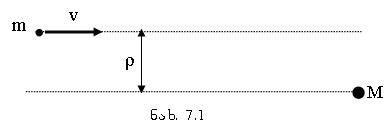
\includegraphics[width=0.5\columnwidth]{figures/fig_1}
           \caption{ამოცანა.}
           %\label{fig:boat1}
        \end{figure}
        
ამოხსნა:	იხსნება იმპულსის მუდმივობისა და ენერგიის მუდმივობით.\\
პასუხი: $$ r_{min} = \frac{1}{v^2} $$

\chapter{მექანიკური რხევები და ტალღები}
\section{რხევის განტოლება}
$$x=x_m\cos(\omega t + \varphi)$$
\section{მათემატიკური ქანქარა}

$$T = 2\pi \sqrt{\dfrac{l}{g}}$$

\section{რეზონანსი}
??

\section{ამოცანები}
\textbf{01.}
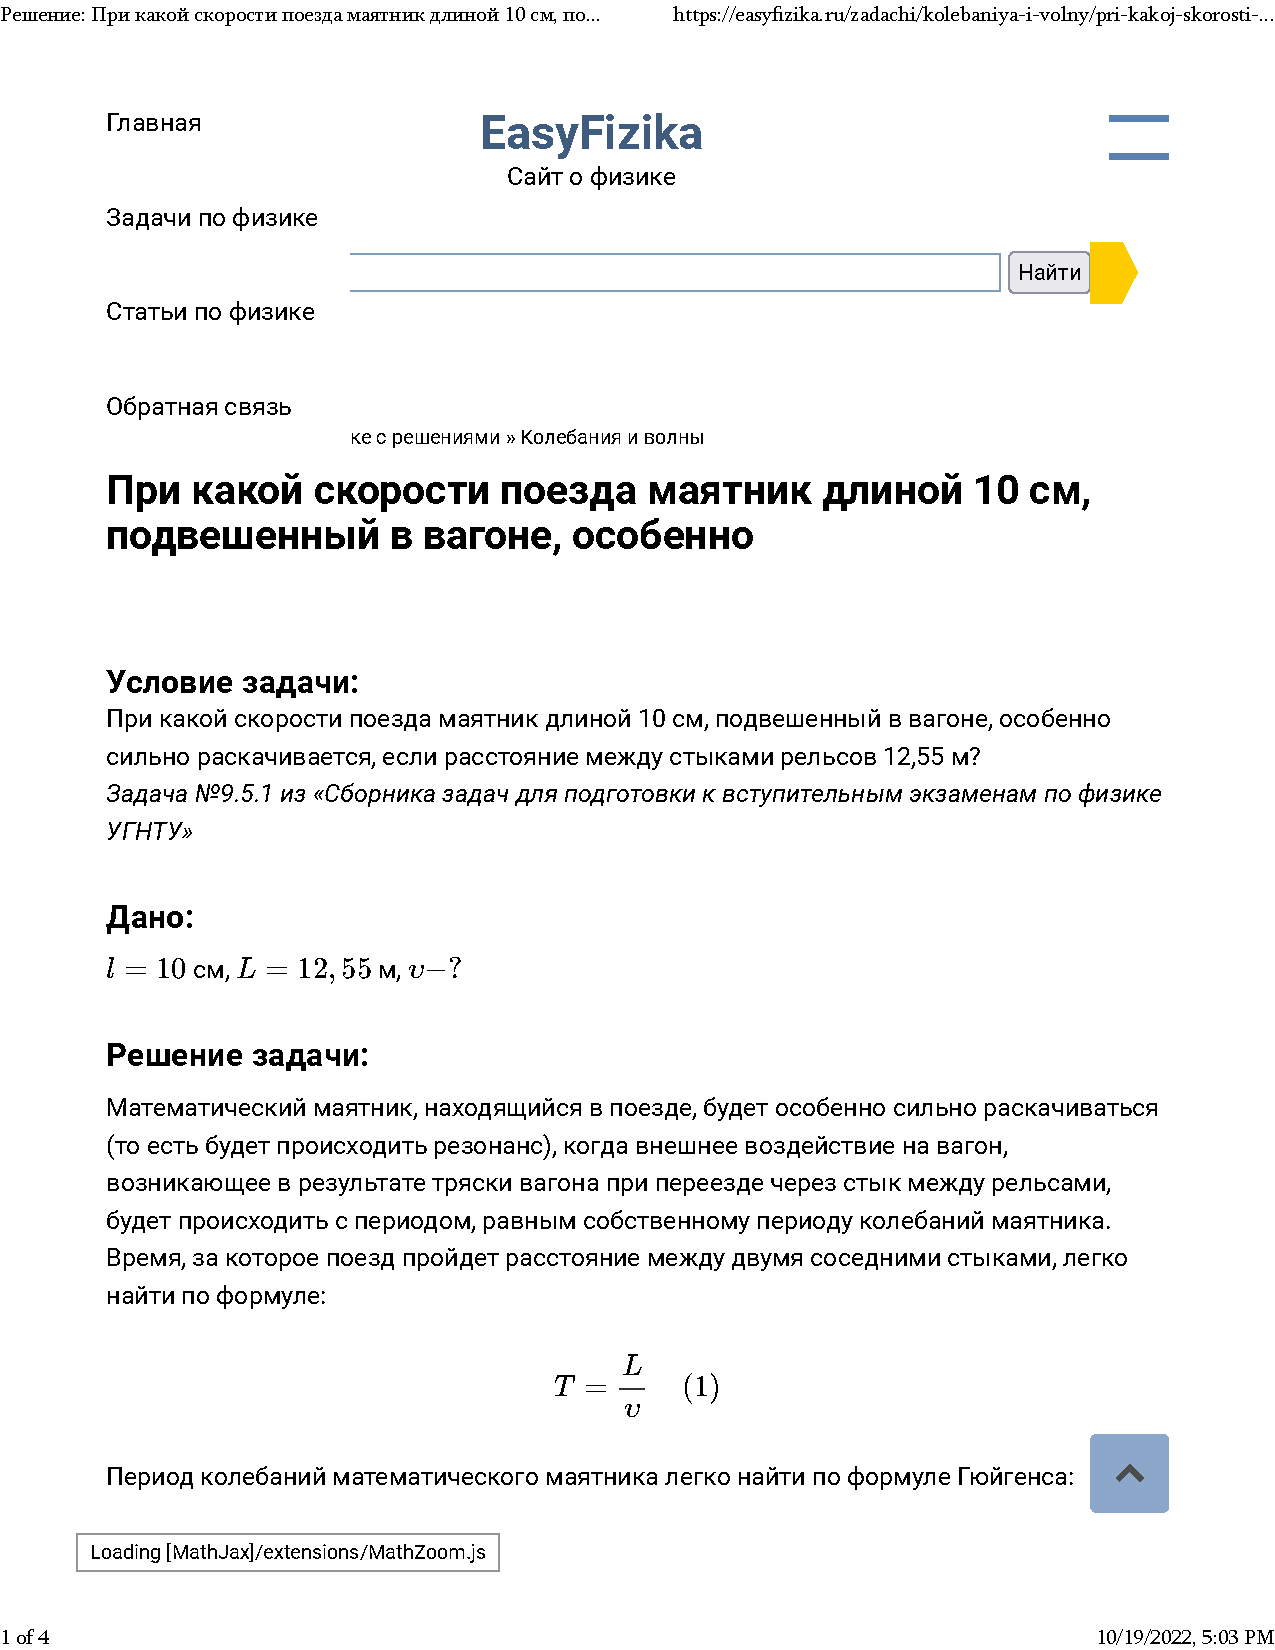
\includegraphics[width=0.9\columnwidth]{temp_pdfs/1.pdf}

\textbf{02.}
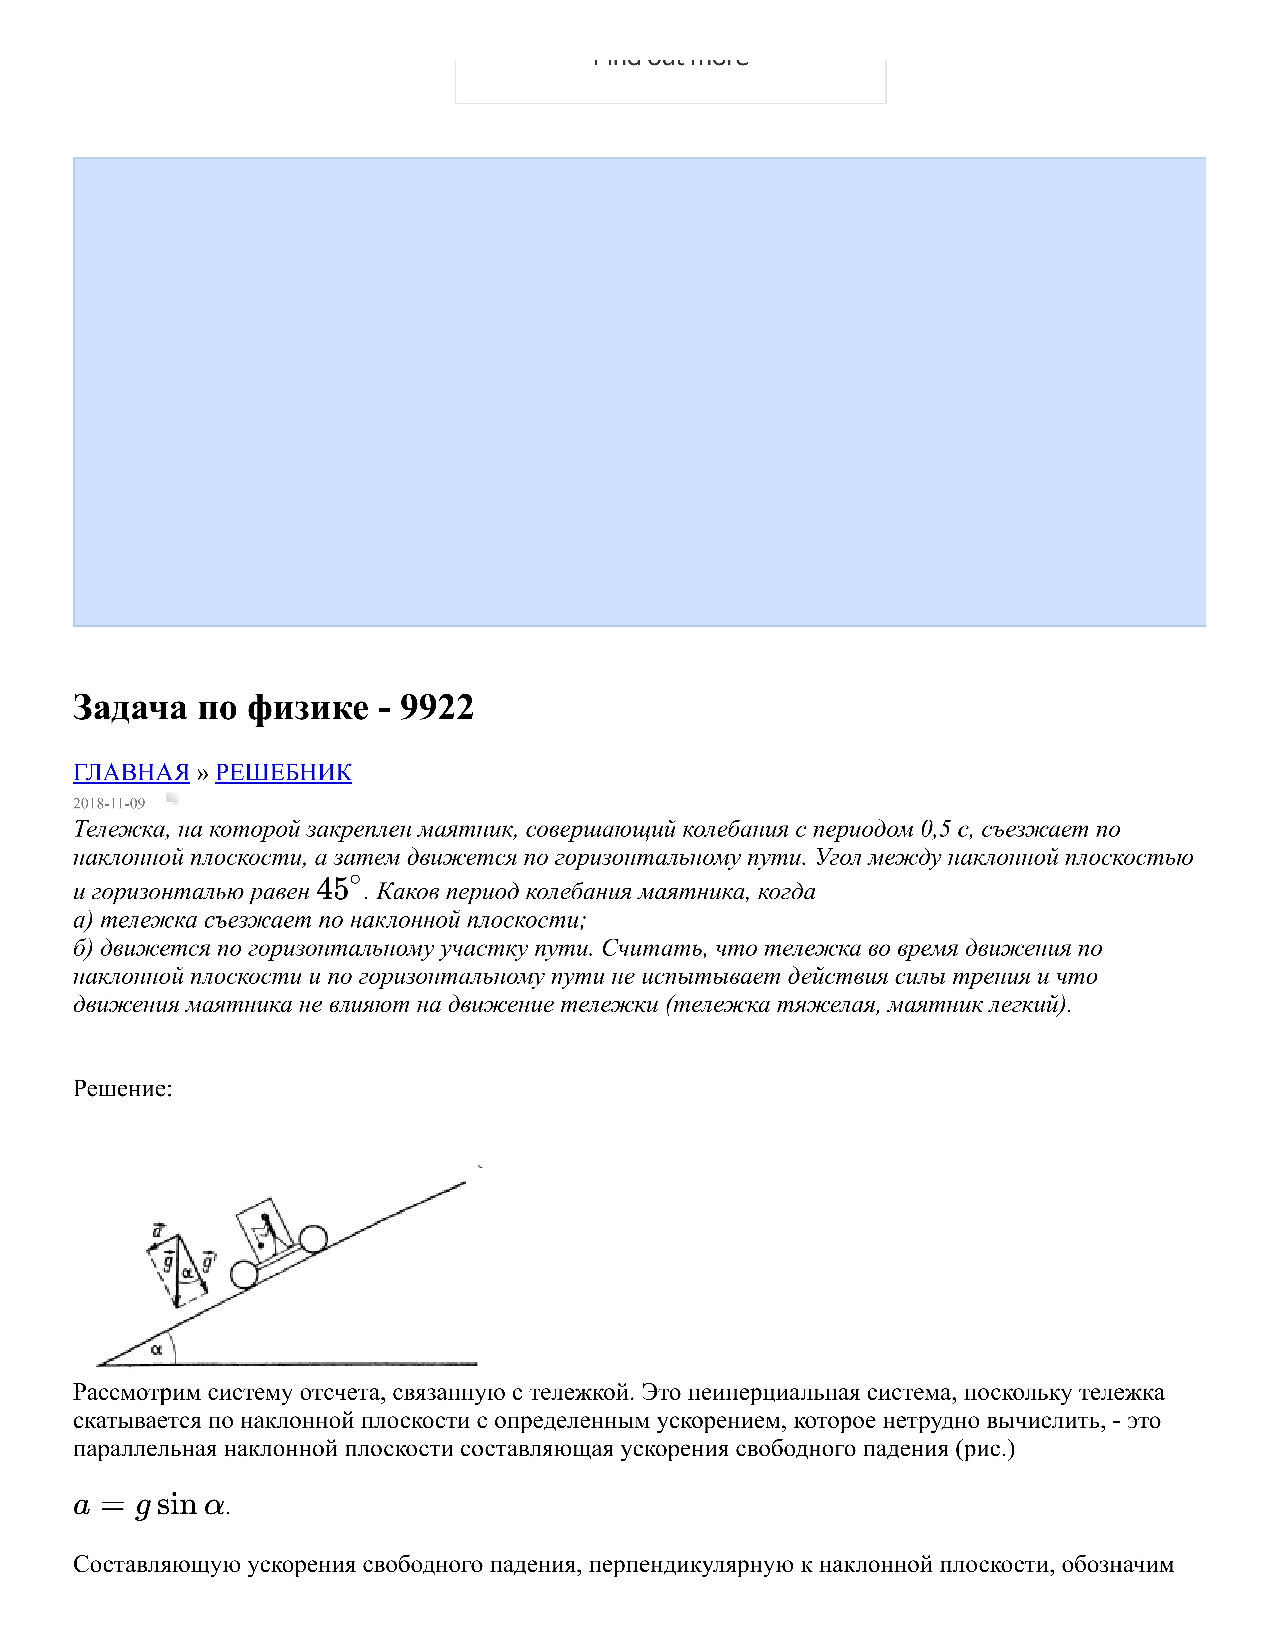
\includegraphics[width=0.9\columnwidth]{temp_pdfs/2.pdf}

\chapter{სითბური მოვლენები}
\section{ენტროპია და მისი კავშირი ალბათობასთა}
%მირინაშვილის მიხედვით. გვერდი 91.
განვიხილოთ ორი სხეული, ენერგიებით $E_1$ და $E_2$,მოცულობებით $V_1$ და $V_2$. მაშინ ამ ორი სხეულის გაერთიანებით მიღებული სისტემისათვის, ენერგია და მოცულობები შეიკრიბება. (ამ სხეულის მოლეკულებს შორს ურთიერთქმედება უგულებელყოფილია).
$$E = E_1 + E_2 \quad V = V_1 + v_2$$
მოდი შევეცადოთ ვიპოვოთ სისტემის ალბათობა, ცალკეული სისტემების ალბათობებით $w_!$ და $w_2$. განვიხილოთ ორი დამოუკიდებელი სხეული $W_1$ და $W_2$ ალბათობების მაკრომდგომარეობით

\section{მენდეელევ-კლაპეირონის განტოლება}
$$PV = \frac{m}{M}RT$$

\section{სითბური ბალანსი}
თუ ნივთიერება დნება $+\lambda m$ გამყარება $-\lambda m$, თუ ნივთიერება ორთქლდება $+r m$ კონდესირდება $-rm$.
\section{ამოცანები.}

\chapter{ელექტრობა}

\section{ემძ-ს შემცველი წრედების გამოთვლა}
როდესაც წრედში გვაქვს ემძ წყარო, აუცილებელია განზოგადებული ომის კანონის გამოყენება. 

$$I = \frac{U_{12} + \mathcal{E}}{r}$$

აქ შემავალი ეს სამი სიდიდე არის ალგებრული ნიშნით, შეიძლება იყოს როგორც უარყოფითი ისე დადებითი, მხოლოდ $r$ არის ცალსახად დადებითი.
\section{გაუსის თეორემა}
შემოვიტანოთ ახალი ფიზიკური სიდიდე - ელექტრული ველის ნაკადი $\Phi$ რაიმე ზედაპირში. განვიხილოთ ერთგვაროვან ელექტრულ ველში მოთავსებული ბრტყელი ზედაპირი. ამ ზედაპირის ფართობი იყოს $S$, ველის დაძაბულობა $\vec{E}$, ხოლო კუთხე დაძაბულობის ვექტორსა და ზედაპირის მართობ $\vec{n}$ ერთეულოვან ვექტორს (ნორმალს) შორის $\alpha$.

ელექტრული ველის ნაკადი ბრტყელ ზედაპირში ტოლია დაძაბულობის მოდულის, ზედაპირის ფართობის და დაძაბულობასა და ზედაპირის ნორმალს შორის კუთხის კოსინუსის ნამრავლის.
	$$\Phi = \vec{E}\cdot S\vec{n}=EScos\alpha=E_n S$$

ნებისმიერ ზედაპირში ელექტრული ნაკადის საპოვნელად ეს ზედაპირი უნდა დავყოთ იმდენად მცირე ელემენტარულ ნაწილებად, რომ თითოეული მათგანი ბრტყლად ჩაითვალოს და ველი მათ ფარგლებში ერთგვაროვნად. თითოეულ ელემენტარულ ზედაპირში ელემენტარულ ნაკადს ვიპოვით (3.1) ფორმულის გამოყენებით. მათი შეკრებით მივიღებთ ნაკადს მთელ ზედაპირში.

სადაც $S_i$ ელემენტარული ზედაპირების ფართობებია, $E_i$ ელემენტების ფარგლებში ველის დაძაბულობის მოდულებია, ხოლო $\alpha_i$ ელემენტების ფარგლებში ველის დაძაბულობასა და ელემენტის ნორმალს შორის კუთხეებია. უფრო ზუსტად, უნდა მოხდეს არა მცირე ელემენტებში ნაკადების აჯამვა, არამედ უსასრულოდ მცირე ელემენტებში ნაკადების ინტეგრება

ჩაკეტილ ზედაპირებში ელექტრული ნაკადის გამოთვლისას ყოველი
ელემენტისათვის იყენებენ გარე ნორმალს.
 
გაუსის თეორემა ამტკიცებს, რომ ელექტრული ველის ნაკადი ნებისმიერ ჩაკეტილ ზედაპირში ტოლია ამ ზედაპირის შიგნით მოთავსებული მუხტების ალგებრული ჯამის ფარდობისა ელექტრულ მუდმივასთან.

$$\Phi = \frac{q}{\epsilon_0}$$

დამტკიცებას ამ ეტაპზე არ მოვიყვანთ.
%ნიკოს ნოუთებში არის დამტკიცება
\section{კონდენსატორი}
კონდენსატორის ენერგია გამოითვლება შემდეგი ფორმულით:
$$C = \frac{q}{\varphi}$$
ბრტყელი კონდენსატორი:
$$C = \frac{\epsilon_0 \epsilon S}{d}$$

\section{ცვლადი დენი}

AC ხასიათდება ორი პარამეტრით: ამპლიტუდა და ფაზით
$$V = IZ$$
1) $V$ და $I$ არის კომპლექსური ძაბვა და ველი. ტრიგონომეტრიულად $A_0cos(\omega t + \theta)$, კომპლექსური ფორმით $A_0exp(\omega t + \theta)$

2) როცა გვაქვს მარტო რეზისტორი $Z=R$, იმპედანსი არის ნამდვილი რიცხვი რომლის მოდული ტოლია წინაღობის.

3) როცა მხოლოდ კონდენსატორია ჩართული, $Z=-\frac{i}{\omega C}$. ეს ნიშნავს რომ იმპედანსი არის წარმოსახვითი რიცხვი. რომლის ტევადობა ტოლია ტევადური წინაღობის.

4) როდესაც გვაქვს მხოლოდ ინდუქტივობა, იმპედანსი არის წარმოსახვითი $Z = + i(\omega L)$ 

5) როცა გვაქვს მიმდევრობითი ჩართვა. $Z = Z_1 + Z_2 + ... + Z_n$

6) როცა პარალელურადაა ჩართული. $\frac{1}{Z} = \frac{1}{Z_1} + \frac{1}{Z_2} + ... + \frac{1}{Z_n}$

\section{ფარადეის კანონები}

ელექტროლიტში დენის გავლისას ელექტროდებზე ნივთიერების გამოყოფის მოვლენას ელექტროლიზი ეწოდება.

ინგლისელმა ფიზიკოსმა ფარადეიმ, ატარებდა რა სხვადასხვა დენს
სხვადასხვა ელექტროლიტში და გულმოდგინედ ზომავდა თითოეული
ელექტროლიტიდან ელექტროდებზე გამოყოფილი ნივთიერების მასას,
1833-1834 წწ. აღმოაჩინა ელექტროლიზის ორი კანონი.

ფარადეის პირველი კანონით დადგენილია დამოკიდებულება ელექტროლიზის დროს გამოყოფილი ნივთიერების მასასა და ელექტროლიტში გავლილ მუხტის სიდიდეს შორის. 

ეს კანონი ასე გამოითქმის: ელექტროლიზის დროს თითოეულ ელექტროდზე გამოყოფილი ნივთიერების მასა ელეკქტროლიტში გავლილი მუხტის სიდიდის პირდაპირ პროპორციულია:

$$m = kIt = kq$$
სადაც $k$ არის ელექტროქიმიური ექვივალენტი.

ქიმიური ექვივალენტი $\frac{M}{n}$
$$k = \frac{1}{F}\frac{M}{n}$$

$F$ ფარადეის მუდმივა $96500$ კ/მოლი

$$m = \frac{1}{F}\frac{M}{n}It$$

\section{გამტარი სფეროები}
წყარო: http://kvant.mccme.ru/pdf/1999/04/kv0499chernoutsan.pdf

%https://tsput.ru/res/fizika/ELECTRO_DREAM/lection_16.html?ysclid=lab5bhhc8c60703496

დამუხტული სფეროს ენერგია, ცალკე ფორმულა და გამოყვანა...

\textbf{ამოცანა 2} ორი გამტარი სფერო რადიუსებით $R_1$ და $R_2$ მოთავსებულია ერთმანეთისაგან შორს. პირველი დამუხტულია $q$ მუხტით, ხოლო მეორე არაა დამუხტული. სფეროები შეაერთეს გრძელი წვრილი მავთულით. რა მუხტები იქნება სფეროებზე შეერთების შემდეგ? რა რაოდენობის სითბო გამოიყოფა სფეროების გადამუხტვის შემდგომ? მავთულის მუხტი არ გაითვალისწინოთ.

\textbf{ამოცანა 3} ორი თხელი კონცენტრული სფერო რადიუსებით $R_1$ და $R_2$ ($R_1$ < $R_2$) და მუხტებით $q_1$ და $q_2$. განსაზღვრეთ სისტემის პოტენციალი და ენერგია. რა მუხტი დარჩება შიდა სფეროზე თუ მას დავამიწებთ? როგორ შეიცვლება ამ დროს სისტემის ენერგია?
	\begin{figure}[H]
		\centering
		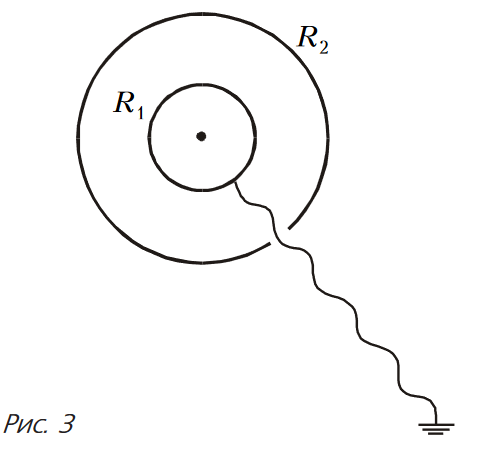
\includegraphics[width=0.3\columnwidth]{figures/Screenshot 2022-11-09 154913}
		\caption{ამოცანა 3.}
		\label{fig:problem_3}
	\end{figure}

\textbf{ამოცანა 5} გამტარი $R$ რადიუსის სფერო დამუხტულია $Q$. რისი ტოლი გახდება სფეროს პოტენციალი, თუ მისი ცენტრიდან $l$ მანძილზე მოვათავსებთ წერტილოვან $q$ მუხტს? განიხილეთ ორი შემთხვევა $l > R$ და $l < R$.

\textbf{ამოცანა 6} მოცემულია ორი კონცენტრული სფერო $R_1$ და $R_2$ ($R_1$ < $R_2$). სფეროებს შორის ცენტრიდან $r$ მანძილზე მოთავსებულია წერტილოვანი $q$ მუხტი. რა მუხტები ექნებათ სფეროებს თუ მათ დავამიწებთ?

\section{რხევითი კონტური და ენერგიის შენახვის კანონები}
%SМ. Бондаров. Колебательный контур и законы сохранения. ¾Квант¿, 2014, No5–6
\textbf{ამოცანა 01.} იდეალური რხევით კონტურში 

\textbf{ამოცანა 02.} ორი ერთნაირი კონდენსატორი $A$ და $B$ ტევადობით $C$, ინდუქტიური კოჭა $L$ ინდუქტივობით, შეერთებულები არიან ისე როგორც ნახაზზეა მოცემული. თავიდან $K$ ჩამრთველი გამორთულია, კონდენსატორი $A$ დამუხტულია $U_0$ ძაბვამდე. კონდენსატორი $B$ არაა დამუხტული, კოჭაში დენი არაა. განსაზღვრეთ მაქსიმალური დენის ძალა ინდუქტიურ კოჭაში, ჩამრთველის ჩართვის შემდგომ.
	\begin{figure}[H]
		\centering
		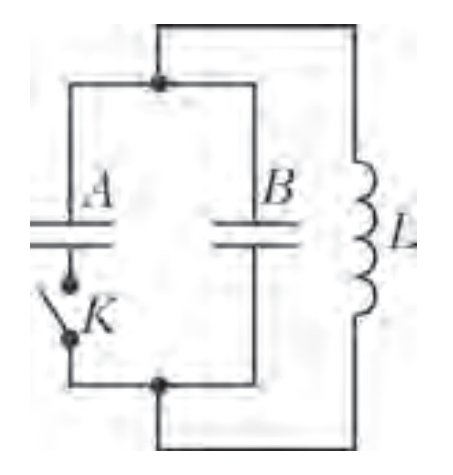
\includegraphics[width=0.2\columnwidth]{figures/Screenshot 2022-11-11 234359}
		\caption{ამოცანა 02.}
		%\label{fig:problem_3}
	\end{figure}

\textbf{ამოცანა 03.} როდესაც $K$ ჩამრთველი ჩაკეტილია $LC$ კონტურში მიმდინარეობს არა მილევადი რხევები. მაშინ როდესაც ძაბვა $C_1$ კონდენსატორზე ძაბვა იყოს მაქსიმალური და ტოლი $U_1$, ჩამრთველს ამორთავენ. განსაზღვრეთ მაქსიმალური დენის ძალა კონტურში ჩამრთველის ამორთვის შემდგომ. ელექტრული კომპონენტების პარამეტრები ნახაზზეა მოცემული.
	\begin{figure}[H]
		\centering
		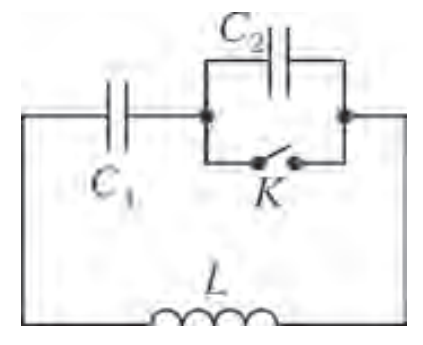
\includegraphics[width=0.2\columnwidth]{figures/Screenshot 2022-11-11 235736}
		\caption{ამოცანა 03.}
		%\label{fig:problem_3}
	\end{figure}

\textbf{ამოცანა 04.} დასამატებელია

\textbf{ამოცანა 05.} როდესაც $K$ ჩამრთველი გახსნილ მდგომარეობაშია $LC$ კონტურში მიმდინარეობს არამილევადი რხევები. მაშინ როდესაც წრედში დენი მაქსიმალურია და ტოლია $I_0$-ის, კეტავენ $K$ ჩამრთველს. განსაზღვრეთ მაქსიმალური ძაბვა კონდენსატორზე ჩამრთველის ჩართვის შემდგომ. კომპონენტების პარამეტრები ნახაზზეა მოცემული.
	\begin{figure}[H]
		\centering
		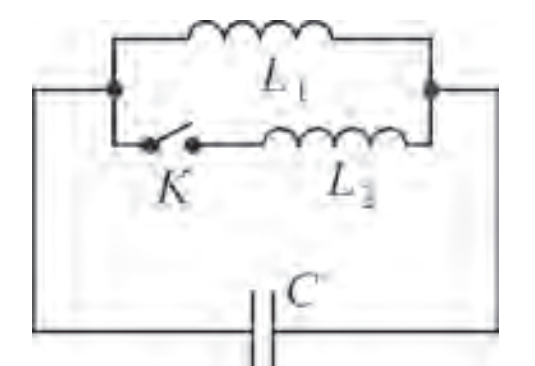
\includegraphics[width=0.2\columnwidth]{figures/Screenshot 2022-11-12 000506}
		\caption{ამოცანა 05.}
		%\label{fig:problem_3}
	\end{figure}

\textbf{ამოცანა 06.} სურათზე გამოსახულ სქემაში წინაღობა არ გვაქვს. $L_1$ და $L_2$ ინდუქტიური კოჭები ერთმანეთთან შეერთებულია მიმდევრობით და $C$ კონდენსატორთან. საწყისს მომენტში $K_1$ და $K_2$ ჩამრთველები გამორთულია. კონდენსატორი დამუხტულია $U_0$ ძაბვამდე. თავიდან რთავენ $K_1$ ჩამრთველს და მას შემდეგ რაც კონდენსატორზე ძაბვა გაუტოლდება ნულს, რთავენ $K_2$ ჩამრთველს. მეორე ჩამრთველის ჩართვიდან გარკვეული დროის შემდგომ კონდენსატორი გადაიმუხტება მაქსიმალურ $U_m$ ძაბვამდე. განსაზღვრეთ ინდუქტივობებში გამავალი დენი $K_2$ ჩართვის მომენტის წინ. ასევე განსაზღვრეთ ძაბვა $U_m$.  
	\begin{figure}[H]
		\centering
		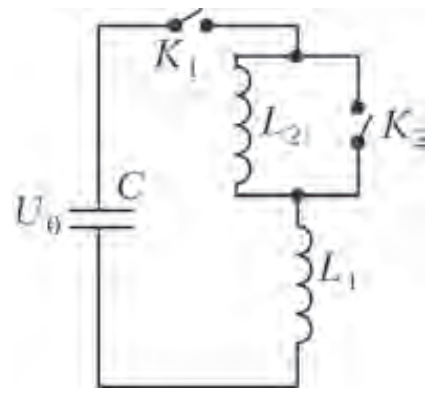
\includegraphics[width=0.2\columnwidth]{figures/Screenshot 2022-11-12 002156}
		\caption{ამოცანა 06.}
		%\label{fig:problem_3}
	\end{figure}

\chapter{გეომეტრიული ოპტიკა}
\section{ჩრდილი და ნახევარჩრდილი} 
თუ სხეულს დავანათებთ წერტილოვანი წყაროდან, მაშინ საგნის ჩრდილი იქნება სრული, მკვეთრად შემოხაზული საზღვრით. 
%https://en.wikipedia.org/wiki/Umbra,_penumbra_and_antumbra#Penumbra
		\begin{figure}[H]
		   \centering
           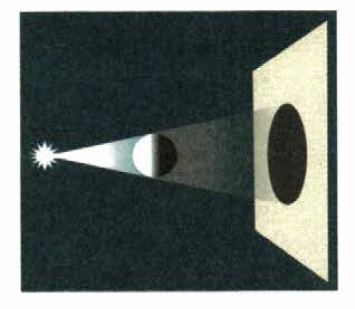
\includegraphics[width=0.3\columnwidth]{figures/shadow}
           \caption{ჩრდილი.}
           \label{fig:shadow}
           %რუსული გენდელშტაინი
        \end{figure}
        
თუკი ობიექტს ვანათებთ არაწერტილოვანი გაწელილი სინათლის წყაროთი, მაშინ ის ასევე წარმოქმნის ნახევარჩრდილს - ნაწილობრივ განათებულ ეკრანის არეს, სადაც მხოლოდ მანათობელი ობიექტის ნაწილიდან ეცემა სინათლე. ზოგიერთ შემთხვევაში შეიძლება სრული ჩრდილი საერთოდ არ გვქონდეს, და მხოლოდ იყოს ნახევარჩრდილი.
		\begin{figure}[H]
		   \centering
           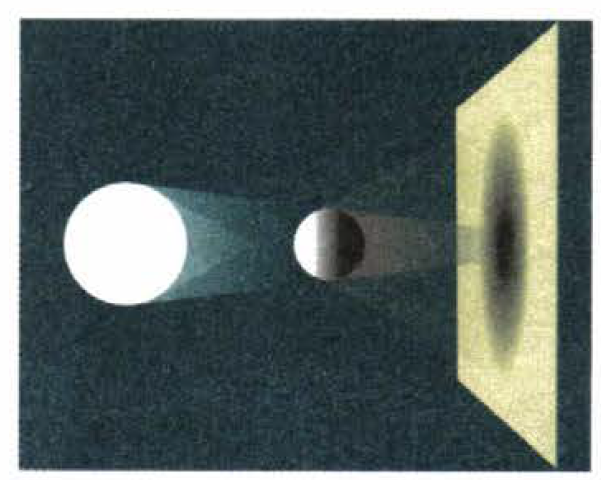
\includegraphics[width=0.3\columnwidth]{figures/penumbra}
           \caption{ნახევარჩრდილი.}
           \label{fig:penumbra}
           %რუსული გენდელშტაინი
        \end{figure}
        
ნახევარჩრდილის ზომის და გეომეტრიული ფორმის განსაზღვრა შესაძლებელია გეომეტრიული აგებით, სინათლის წრფივი გავრცელების მიხედვით.

\section{თხელი ლინზები} ლინზას ორი სფერული ზედაპირით შემოსაზღვრულ გამჭვირვალე სხეულს უწოდებენ. თუ მისი სისქე მცირეა სფერული ზედაპირების სიმრუდის რადიუსთან შედარებით, მაშინ ლინზას თხელს უწოდებენ \ref{fig:thin_lenses}.
		\begin{figure}[h]
		   \centering
           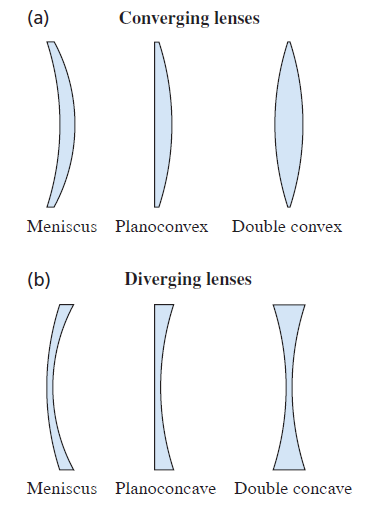
\includegraphics[width=0.4\columnwidth]{figures/thin_lenses}
           \caption{სხივთა სვლა თხელ ა) შემკრებ, ბ) გამბნევ ლინზაში.}
           \label{fig:thin_lenses}
        \end{figure}


ლინზები პრაქტიკულად ყველა ოპტიკური ხელსაწყოს შემადგენლობაში შედიან. არსებობს შემკრები და გამბნევი ლინზები. შემკრები ლინზა შუაში უფრო სქელია ვიდრე კიდეებზე, გამბნევი კი პირიქით, შუაშია უფრო თხელი.

თხელი ლინზის ფორმულა
	\begin{equation}
		\frac{1}{f} + \frac{1}{d} = \frac{1}{F}
	\end{equation}

$D$ სიდიდე ფოკუსური მანძილის შებრუნებულია და ლინზის ოპტიკურ ძალას უწოდებენ. ოპტიკური ძალის ერთეულია დიოპტრი. დიოპტრი ერთი მეტრი ფოკუსური მანძილის მქონე ლინზის ოპტიკური ძალაა:

%	\begin{tabular}{ |c|c|c| }
%		\centering
%		\hline
%		სიდიდე & ნიშანი & col3 \\
%		\hline
%		გამოსახულება & წარმოსახვითი & - \\ 
%		\hline
%	\end{tabular}

\section{გამოსახულების აგება ლინზებსა და სფერულ სარკეებში}
ლინზით ან სარკით მიღებული გამოსახულების ადგილმდებარეობის განსაზღვრა შეიძლება ორი მეთოდით - ალგებრული გამოთვლით (ლინზისა და სარკის ფორმულის გამოყენებით) ანდა გეომეტრიული აგებით.

პირველი მეთოდი თუმც არის უფრო უნივერსალური, ხშირად რთულ ოპტიკურ სისტემებში მას თავს ვერ ავარიდებთ. სამაგიეროდ მეორე მეთოდი უფრო თვალსაჩინოა. ამიტომაც ალგებრულად ამოცანის შემთხვევაშიც კი ვაკეთებთ ნახაზს, რომელიც გვეხმარება საჭირო სისტემის დაწერაში. თუ ამოცანა არ არის ზედმეტად შრომატევადი(?), აგებით ამოხსნა არის უფრო მოსახერხებელი.

თხელ ლინზებში გამოსახულების აგებისას ვსარგებლობთ სამი ძირითადი თვისებით სინათლის სხივის ნახ.ა)~\ref{fig:optics_1}.
		\begin{figure}[h]
		   \centering
           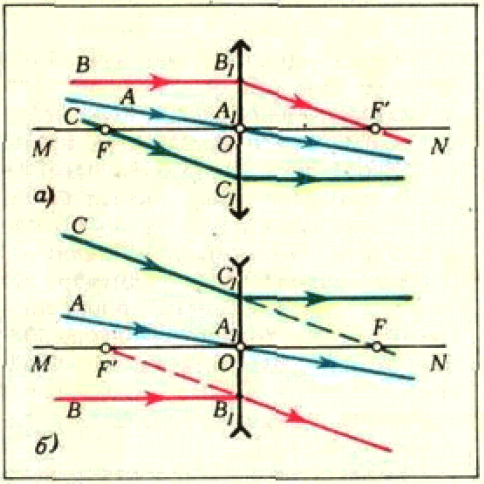
\includegraphics[width=0.5\columnwidth]{figures/optics_1}
           \caption{სხივთა სვლა თხელ ა) შემკრებ, ბ) გამბნევ ლინზაში.}
           \label{fig:optics_1}
        \end{figure}

1) სხივი $AA_1$, რომელიც გადის ლინზის ოპტიკურ ცენტრში $O$ (მეორენაირად ეძახიან დამხმარე ოპტიკურ ღერძს) არ გარდატყდება.

2) სხივი $BB_1$,რომელიც ეცემა ლინზას მთავარი ოპტიკური ღერძის პარალელურად გარდატყდება და გაივლის ლინზის უკანა $F'$ ფოკუსსი.

3) სხივი $CC_1$, რომელიც გადის წინა ფოკუსში $F$, ლინზაში გარდატეხის მერე გამოდის მთავარი ოპტიკური ღერძის პარალელურად.

უკანა ფოკუსი $F'$ ეწოდება წერტილს რომელშიც იკრიბებიან გარდატეხის შემდგომ ოპტიკური ღერძის პარალელურად,ლინზაზე დაცემული სხივები. წინა $F$ და უკანა $F'$ ფოკუსები განლაგებულები არიან თხელი ლინზის მიმართ სიმეტრიულად. $F$ გადის უკანა ფოკალური სიბრტზე, $F'$-ში გადის უკანა ფოკალური სიბრტყე.

ხანდახან ასევე გვეხმარება შემდეგი წესებიც:
1) სხივები, რომლებიც ლინზას ეცემიან პარალელურ ნაკადად, გარდატეხის შემდეგ იკრიბებიან უკანა ფოკალურ სიბრტყეში~\ref{fig:optics_2}.

2) სხივები რომლებიც გამოდიან ლინზიდან პარალელურ ნაკადად, ლინზაზე დაცემამდე გადაიკვეთნენ წინა ფოკალურ სიბრტყეში~\ref{fig:optics_3}. 

		\begin{figure}[h]
		   \centering
           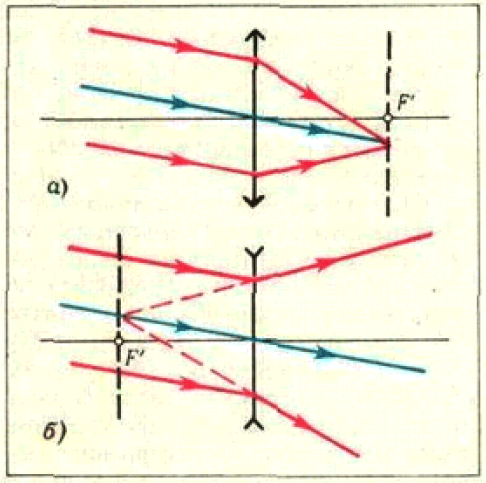
\includegraphics[width=0.5\columnwidth]{figures/optics_2}
           \caption{ლინზაზე დაცემულ პარალელურ სხივთა სვლა თხელ ა) შემკრებ, ბ) გამბნევ ლინზაში.}
           \label{fig:optics_2}
        \end{figure}

		\begin{figure}[h]
		   \centering
           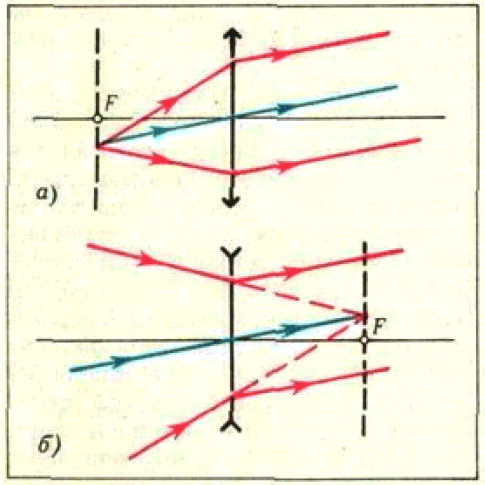
\includegraphics[width=0.5\columnwidth]{figures/optics_3}
           \caption{ლინზიდან გამოსული პარალელურ სხივთა "უკუსვლა" თხელ ა) შემკრებ, ბ) გამბნევ ლინზაში.}
           \label{fig:optics_3}
        \end{figure}

\begin{table}[]
\begin{tabular}{|lllll|}
\hline
\multicolumn{5}{|c|}{\textbf{შემკრები ლინზა (f)}}                                                                                                                                        \\ \hline
\multicolumn{1}{|l|}{\textbf{სხეული ($d_o$)}} & \multicolumn{4}{l|}{\textbf{გამოსახულება ($d_i$)}}                                                                                       \\ \hline
\multicolumn{1}{|l|}{\textbf{მდებარეობა}}     & \multicolumn{1}{l|}{\textbf{ტიპი}} & \multicolumn{1}{l|}{\textbf{მდებარეობა}} & \multicolumn{1}{l|}{\textbf{ორიენტაცია}} & \textbf{ზომა} \\ \hline
\multicolumn{1}{|l|}{}                        & \multicolumn{1}{l|}{ნამდვილი}      & \multicolumn{1}{l|}{}                    & \multicolumn{1}{l|}{შებრუნებული}         & შემცირებული   \\ \hline
\multicolumn{1}{|l|}{}                        & \multicolumn{1}{l|}{ნამდვილი}      & \multicolumn{1}{l|}{}                    & \multicolumn{1}{l|}{შებრუნებული}         & იგივე ზომის   \\ \hline
\multicolumn{1}{|l|}{}                        & \multicolumn{1}{l|}{ნამდვილი}      & \multicolumn{1}{l|}{}                    & \multicolumn{1}{l|}{შებრუნებული}         & გადიდებული    \\ \hline
\multicolumn{1}{|l|}{}                        & \multicolumn{1}{l|}{}              & \multicolumn{1}{l|}{}                    & \multicolumn{1}{l|}{}                    &               \\ \hline
\multicolumn{1}{|l|}{}                        & \multicolumn{1}{l|}{წარმოსახვითი}  & \multicolumn{1}{l|}{}                    & \multicolumn{1}{l|}{პირდაპირი}           & გადიდებული    \\ \hline
\end{tabular}
\end{table}

\section{სფერული სარკე}

\section{მარგველაშვილი}
\textbf{6-118.} პარალელურ სხივთა კონა ეცემა შემკრებ ლინზას, რომლის ფოკუსური მანძილია 20 სმ. ლინზიდან რა მანძილზე უნდა მოვათავსოთ მეორე ასეთივე ლინზა, რომ მისგან გამოსული სხივები ისევ პარალელური იყოს?

6--119. შემკრებ ლინზას, რომლის ფოკუსური მანძილია. 20 (გ
ეცემა პარალელურ სხივთა კონა. ლინზის ოპტიკურ ღერთე მისგან
60 სმ მანძილზე მოთავსებულია მეორე შემკრები ლინზა, რომ
ნაც კვლავ პარალელური სხივები გამოდის. იპოვეთ მეორე ლიზას
ფოკუსური მანძილი.

6--190. გამბნევი ლინზის ფოკუსური მანძილია 7 სმ. რა მანძილზე
უნდა დავაყენოთ შემკრები ლინზა, რომლის ფოკუსური მანძილია 20
სმ, რომ მივიღოთ პარალელური სხივები, თუ გამბნევ ლინზახ ეცემა
პარალელური სხივები?

6--181. მილში მოთავსებულია ორი შემკრები ლინზა, რომლებიც
ერთმანეთისაგან დაშორებულია 16 სმ-ით. პირველი ლინზის ფოკე-
სური მანძილია 8 სმ, მეორისა –– 5 სმ. საგანი მდებარეობს პირველი
ლინზიდან 40 სმ მანძილზე, მეორე ლინზიდან რა მანძილზე მიიღება
გამოსახულება?

9--199. შემკრებ ლინზას ეცემა მთავარი ოპტიკური ღერძის პარ»-
ლელური სხივთა კონა. შემკრები ლინზიდან 10 სმ-ის მანძიღბე ი
თავსებულია გამბნევი ლინხა. გამბნევი ლინზიდან რა მანი ე. 20
იღება გამოსახულება, თუ შემკრები ლინზის ფოკუსური მანძილ
სმ, გამბნევისა კი –– 15 სმ. ს პარ»

\section{ამოცანები.}

\textbf{რიმკევიჩი 1075} რამდენით გაიზრდება კუთხე დაცემულ და არეკვლილ სხივებს შორის, თუ ბრტყელ სარკეს $\phi$ კუთხით შემოვაბრუნებთ ღერძის გარშემო, რომელიც სხივის არეკვლის წერტილში გადის და სხიგების განლაგების სიბრტყის მართობია?

\textbf{რიმკევიჩი 1076} დახაზეთ ორი ურთიერთმართობი $AO$ და $OB$ სარკე. $OB$ სარკეზე დაცემული $CD$ სხივი ღა სხივის შემდგომი სვლის $DE$ და $EF$ მიმართულებები. დაამტკიცეთ, რომ $EF$ სხივი $CD$-ს პარალელურია, $CD$ სხივის ნებისმიერი კუთხით დაცემისას.

\textbf{რიმკევიჩი 1083} რა $h$ სიმაღლეზე იმყოფება $A$ აეროსტატი, თუ $H$ სიმაღლის კოშკიდან იგი ჰორიზონტისადმი $\alpha$ კუთხით ჩანს, ხოლო მისი გამოსახულება ტბაში ჰორიზონტისადმი $\beta$ კუთხით ჩანს.
		\begin{figure}[h]
		   \centering
           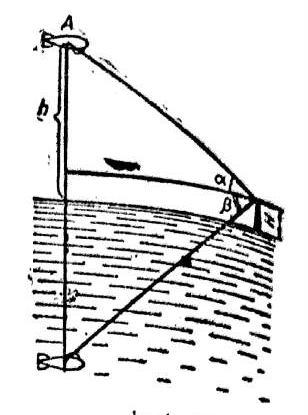
\includegraphics[width=0.5\columnwidth]{figures/1083}
           \caption{.}
           \label{fig:1083}
        \end{figure}

\textbf{რიმკევიჩი 1097} 2 მ სიღრმის წყალსაცავის ფსკერზე ჩასობილია ხიმინჯი, რომელიც წყლის ზედაპირიდან 0.5 მ-ზეა ამოშვერილი. იპოვეთ ხიმინჯის ჩრდილის სიგრძე წყალსაცავის ფსკერზე, თუ სხივები $30 \degree$-იანი კუთხით ეცემიან.

\textbf{რიმკევიჩი 1101} . იპოვეთ პარალელურწახნაგებიან გამჭვირვალე ფირფიტაში გამავალი სხივის $a$ წანაცვლება, თუ სხივის დაცემის კუთხეა $\alpha$, გარდატეხის კუთხე $\gamma$, ხოლო ფირფიტის სისქე $d$. მეიძლება თუ არა ამ ფირფიტაში გამავალმა სხივმა წაინაცვლოს ისე, რომ მის მიმართულებასა და პირვანდელ მიმართულებას შორის მანძილი ფირფიტის სისქეზე მეტი აღმოჩნდეს?

\textbf{..} 
ორ ბრტყელ სარკეს შორის კუთხე არის $\alpha$. იპოვეთ სარკეებს შორის მოთავსებული მნათი წერტილის რამდენი გამოსახულება მიიღება ასეთ სარკეში.

\textbf{01.}
%იროდოვი 216
როგორია დაცემის კუთხე, თუ წყლის ზედაპირიდან არეკვლილი სხივი გარდატეხილი სხივის პერპენდიკულარულია.

\textbf{02.}
%იროდოვი 218
სინათლის სხივი ეცემა $d = 0.6$ სმ სისქის ბრტყელი პარალელური მინის ფირფიტას.დაცემის კუთხე $60 \degree$-ია. იპოვეთ ამ ფირფიტაში გასული სხივის წანაცვლების სიდიდე.

\textbf{217}
იროდოვი 
მოცემულია ორი ბრტყელი საზღვრის მქონე ორი ოპტიკური გარემო. დავუშვათ რომ სხივის დაცემის ზღვრული კუთხე $\theta_1$-ის ტოლია, ხოლო ხ არის დაცემის კუთხე, რომლის დროსაც გარდატეხილი სხივი არეკვლილი სხივის პერპენდიკულარულია (იგულისხმება რომ სხივი ვრცელდება ოპტიკურად მეტად მკვრივი გარემოდან). იპოვეთ ამ ორი გარემოს ფარდობიდითი გარდატეხის მაჩვენებელი, თუ $\eta = 1.28$.

\begin{table}[]
\begin{tabular}{|lllll|}
\hline
\multicolumn{5}{|c|}{\textbf{შემკრები ლინზა (f)}}                                                                                                                                                                        \\ \hline
\multicolumn{1}{|l|}{\textbf{სხეული ($d_o$)}}                                 & \multicolumn{4}{c|}{\textbf{გამოსახულება ($d_i$)}}                                                                                       \\ \hline
\multicolumn{1}{|l|}{\textbf{მდებარეობა}}                                     & \multicolumn{1}{l|}{\textbf{ტიპი}} & \multicolumn{1}{l|}{\textbf{მდებარეობა}} & \multicolumn{1}{l|}{\textbf{ორიენტაცია}} & \textbf{ზომა} \\ \hline
\multicolumn{1}{|l|}{$\infty \textgreater d\_o \textgreater 2f$} & \multicolumn{1}{l|}{ნამდვილი}      & \multicolumn{1}{l|}{}                    & \multicolumn{1}{l|}{შებრუნებული}         & შემცირებული   \\ \hline
\multicolumn{1}{|l|}{$d_o = 2f$}                                               & \multicolumn{1}{l|}{ნამდვილი}      & \multicolumn{1}{l|}{d\_i = 2f}           & \multicolumn{1}{l|}{შებრუნებული}         & იგივე ზომის   \\ \hline
\multicolumn{1}{|l|}{$2f < d_o < f$}                           & \multicolumn{1}{l|}{ნამდვილი}      & \multicolumn{1}{l|}{}                    & \multicolumn{1}{l|}{შებრუნებული}         & გადიდებული    \\ \hline
\multicolumn{1}{|l|}{$d_o = f$}                                                & \multicolumn{1}{l|}{}              & \multicolumn{1}{l|}{}                    & \multicolumn{1}{l|}{}                    &               \\ \hline
\multicolumn{1}{|l|}{$d_o < f$}                                        & \multicolumn{1}{l|}{წარმოსახვითი}  & \multicolumn{1}{l|}{}                    & \multicolumn{1}{l|}{პირდაპირი}           & გადიდებული    \\ \hline
\end{tabular}
\end{table}

\chapter{ფიზიკური ოპტიკა}


	\begin{figure}[H]
    	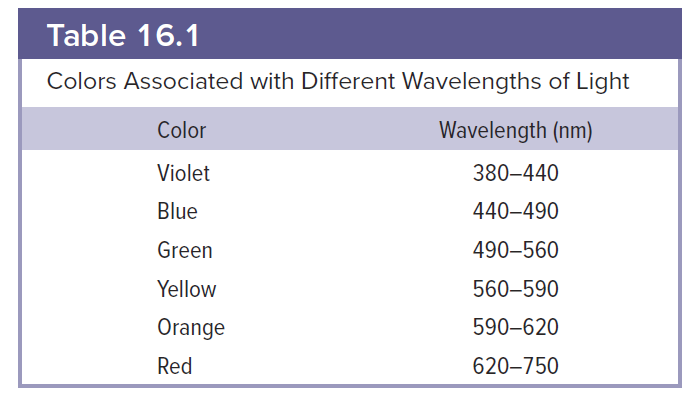
\includegraphics[width=0.8\columnwidth]{figures/yyyu}
    \caption{A boat.}
    \label{fig:02}
    \end{figure}


\chapter{ბირთვული ფიზიკა}
$\alpha$ დაშლა $\ce{^235_92U -> ^231_90Th + ^4_2He}$

რადიოაქტიურობა - როცა ბირთვი იყოფა თვითონ ბირთვი
ბირთვული რეაქციები - როცა ბირთვი ურთიერთქმედებს სხვა ბირთვთან ან ნაწილაკთან.

\chapter{მათემატიკური ნაწილი}
\section{წარმოებულები}
\section{ინტეგრალები}
https://calculus.nipissingu.ca/tutorials/integrals.html

\chapter{მელედინი 1.165} აუზის პორიზონტალურ ზედაპირზე დევს უმასო $r$ რადიუსის სფერო, რომელზეც მობმულია წვრილი $l$ სიგრძის ღერო, რომელიც ეხება აუზის ფსკერს, იხილე ნახაზი. იპოვეთ უმცირესი ღეროს მასა რომლისთვისაც სფერო ჯერ კიდევ დევს ფსკერზე. სითხის სიმკვრივეა $\rho_0$. 

\end{document}
